% Options for packages loaded elsewhere
\PassOptionsToPackage{unicode}{hyperref}
\PassOptionsToPackage{hyphens}{url}
%
\documentclass[
]{article}
\usepackage{amsmath,amssymb}
\usepackage{lmodern}
\usepackage{iftex}
\ifPDFTeX
  \usepackage[T1]{fontenc}
  \usepackage[utf8]{inputenc}
  \usepackage{textcomp} % provide euro and other symbols
\else % if luatex or xetex
  \usepackage{unicode-math}
  \defaultfontfeatures{Scale=MatchLowercase}
  \defaultfontfeatures[\rmfamily]{Ligatures=TeX,Scale=1}
\fi
% Use upquote if available, for straight quotes in verbatim environments
\IfFileExists{upquote.sty}{\usepackage{upquote}}{}
\IfFileExists{microtype.sty}{% use microtype if available
  \usepackage[]{microtype}
  \UseMicrotypeSet[protrusion]{basicmath} % disable protrusion for tt fonts
}{}
\makeatletter
\@ifundefined{KOMAClassName}{% if non-KOMA class
  \IfFileExists{parskip.sty}{%
    \usepackage{parskip}
  }{% else
    \setlength{\parindent}{0pt}
    \setlength{\parskip}{6pt plus 2pt minus 1pt}}
}{% if KOMA class
  \KOMAoptions{parskip=half}}
\makeatother
\usepackage{xcolor}
\IfFileExists{xurl.sty}{\usepackage{xurl}}{} % add URL line breaks if available
\IfFileExists{bookmark.sty}{\usepackage{bookmark}}{\usepackage{hyperref}}
\hypersetup{
  pdftitle={Weather and fuel as modulators of grassland fire behavior in the northern Great Plains},
  pdfauthor={DA McGranahan, ME Zopfi, KA Yurkonis},
  hidelinks,
  pdfcreator={LaTeX via pandoc}}
\urlstyle{same} % disable monospaced font for URLs
\usepackage[margin=1in]{geometry}
\usepackage{color}
\usepackage{fancyvrb}
\newcommand{\VerbBar}{|}
\newcommand{\VERB}{\Verb[commandchars=\\\{\}]}
\DefineVerbatimEnvironment{Highlighting}{Verbatim}{commandchars=\\\{\}}
% Add ',fontsize=\small' for more characters per line
\usepackage{framed}
\definecolor{shadecolor}{RGB}{248,248,248}
\newenvironment{Shaded}{\begin{snugshade}}{\end{snugshade}}
\newcommand{\AlertTok}[1]{\textcolor[rgb]{0.94,0.16,0.16}{#1}}
\newcommand{\AnnotationTok}[1]{\textcolor[rgb]{0.56,0.35,0.01}{\textbf{\textit{#1}}}}
\newcommand{\AttributeTok}[1]{\textcolor[rgb]{0.77,0.63,0.00}{#1}}
\newcommand{\BaseNTok}[1]{\textcolor[rgb]{0.00,0.00,0.81}{#1}}
\newcommand{\BuiltInTok}[1]{#1}
\newcommand{\CharTok}[1]{\textcolor[rgb]{0.31,0.60,0.02}{#1}}
\newcommand{\CommentTok}[1]{\textcolor[rgb]{0.56,0.35,0.01}{\textit{#1}}}
\newcommand{\CommentVarTok}[1]{\textcolor[rgb]{0.56,0.35,0.01}{\textbf{\textit{#1}}}}
\newcommand{\ConstantTok}[1]{\textcolor[rgb]{0.00,0.00,0.00}{#1}}
\newcommand{\ControlFlowTok}[1]{\textcolor[rgb]{0.13,0.29,0.53}{\textbf{#1}}}
\newcommand{\DataTypeTok}[1]{\textcolor[rgb]{0.13,0.29,0.53}{#1}}
\newcommand{\DecValTok}[1]{\textcolor[rgb]{0.00,0.00,0.81}{#1}}
\newcommand{\DocumentationTok}[1]{\textcolor[rgb]{0.56,0.35,0.01}{\textbf{\textit{#1}}}}
\newcommand{\ErrorTok}[1]{\textcolor[rgb]{0.64,0.00,0.00}{\textbf{#1}}}
\newcommand{\ExtensionTok}[1]{#1}
\newcommand{\FloatTok}[1]{\textcolor[rgb]{0.00,0.00,0.81}{#1}}
\newcommand{\FunctionTok}[1]{\textcolor[rgb]{0.00,0.00,0.00}{#1}}
\newcommand{\ImportTok}[1]{#1}
\newcommand{\InformationTok}[1]{\textcolor[rgb]{0.56,0.35,0.01}{\textbf{\textit{#1}}}}
\newcommand{\KeywordTok}[1]{\textcolor[rgb]{0.13,0.29,0.53}{\textbf{#1}}}
\newcommand{\NormalTok}[1]{#1}
\newcommand{\OperatorTok}[1]{\textcolor[rgb]{0.81,0.36,0.00}{\textbf{#1}}}
\newcommand{\OtherTok}[1]{\textcolor[rgb]{0.56,0.35,0.01}{#1}}
\newcommand{\PreprocessorTok}[1]{\textcolor[rgb]{0.56,0.35,0.01}{\textit{#1}}}
\newcommand{\RegionMarkerTok}[1]{#1}
\newcommand{\SpecialCharTok}[1]{\textcolor[rgb]{0.00,0.00,0.00}{#1}}
\newcommand{\SpecialStringTok}[1]{\textcolor[rgb]{0.31,0.60,0.02}{#1}}
\newcommand{\StringTok}[1]{\textcolor[rgb]{0.31,0.60,0.02}{#1}}
\newcommand{\VariableTok}[1]{\textcolor[rgb]{0.00,0.00,0.00}{#1}}
\newcommand{\VerbatimStringTok}[1]{\textcolor[rgb]{0.31,0.60,0.02}{#1}}
\newcommand{\WarningTok}[1]{\textcolor[rgb]{0.56,0.35,0.01}{\textbf{\textit{#1}}}}
\usepackage{graphicx}
\makeatletter
\def\maxwidth{\ifdim\Gin@nat@width>\linewidth\linewidth\else\Gin@nat@width\fi}
\def\maxheight{\ifdim\Gin@nat@height>\textheight\textheight\else\Gin@nat@height\fi}
\makeatother
% Scale images if necessary, so that they will not overflow the page
% margins by default, and it is still possible to overwrite the defaults
% using explicit options in \includegraphics[width, height, ...]{}
\setkeys{Gin}{width=\maxwidth,height=\maxheight,keepaspectratio}
% Set default figure placement to htbp
\makeatletter
\def\fps@figure{htbp}
\makeatother
\setlength{\emergencystretch}{3em} % prevent overfull lines
\providecommand{\tightlist}{%
  \setlength{\itemsep}{0pt}\setlength{\parskip}{0pt}}
\setcounter{secnumdepth}{-\maxdimen} % remove section numbering
\usepackage{amsmath}
\renewcommand{\familydefault}{\sfdefault}
\usepackage{hyperref}
\usepackage{booktabs}
\ifLuaTeX
  \usepackage{selnolig}  % disable illegal ligatures
\fi

\title{Weather and fuel as modulators of grassland fire behavior in the
northern Great Plains}
\usepackage{etoolbox}
\makeatletter
\providecommand{\subtitle}[1]{% add subtitle to \maketitle
  \apptocmd{\@title}{\par {\large #1 \par}}{}{}
}
\makeatother
\subtitle{Supplementary information}
\author{DA McGranahan, ME Zopfi, KA Yurkonis}
\date{2022-05-12}

\begin{document}
\maketitle

\hypertarget{study-locations}{%
\section{Study locations}\label{study-locations}}

\begin{figure}

{\centering 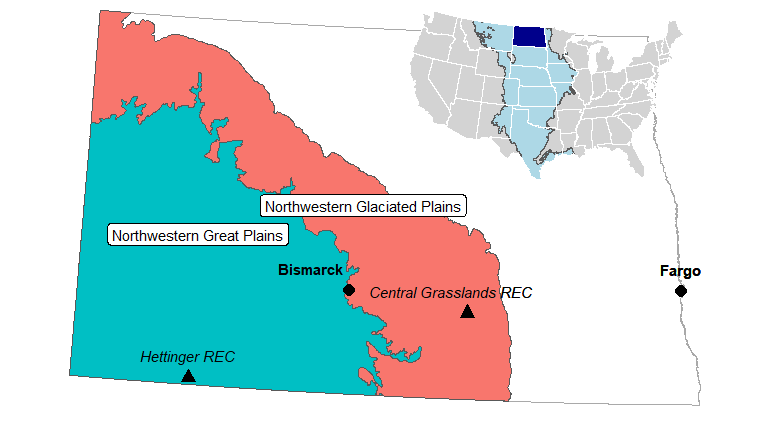
\includegraphics[width=1\linewidth]{figures/map} 

}

\caption{Main map: Study locations (triangles) within two EPA level 3 ecoregions in North Dakota. Inset: State of North Dakota (dark blue) within the Great Plains (light blue) with respect to the continental United States. \label{fig:map}}\label{fig:unnamed-chunk-1}
\end{figure}
\clearpage

\hypertarget{data-collection}{%
\section{Data collection}\label{data-collection}}

For even more information about the FeatherFlame datalogger system,
please see:

\begin{itemize}
\item
  McGranahan DA (2021) FeatherFlame: An Arduino-based thermocouple
  datalogging system to record wildland fire flame temperatures
  \emph{in agris}. Rangeland Ecology \& Management 76, 43--47
  \href{https://doi.org/10.1016/j.rama.2021.01.008}{DOI:
  10.1016/j.rama.2021.01.008}
\item
  \href{https://diyfirescience.info}{diyfirescience.info}
\end{itemize}

\begin{figure}

{\centering 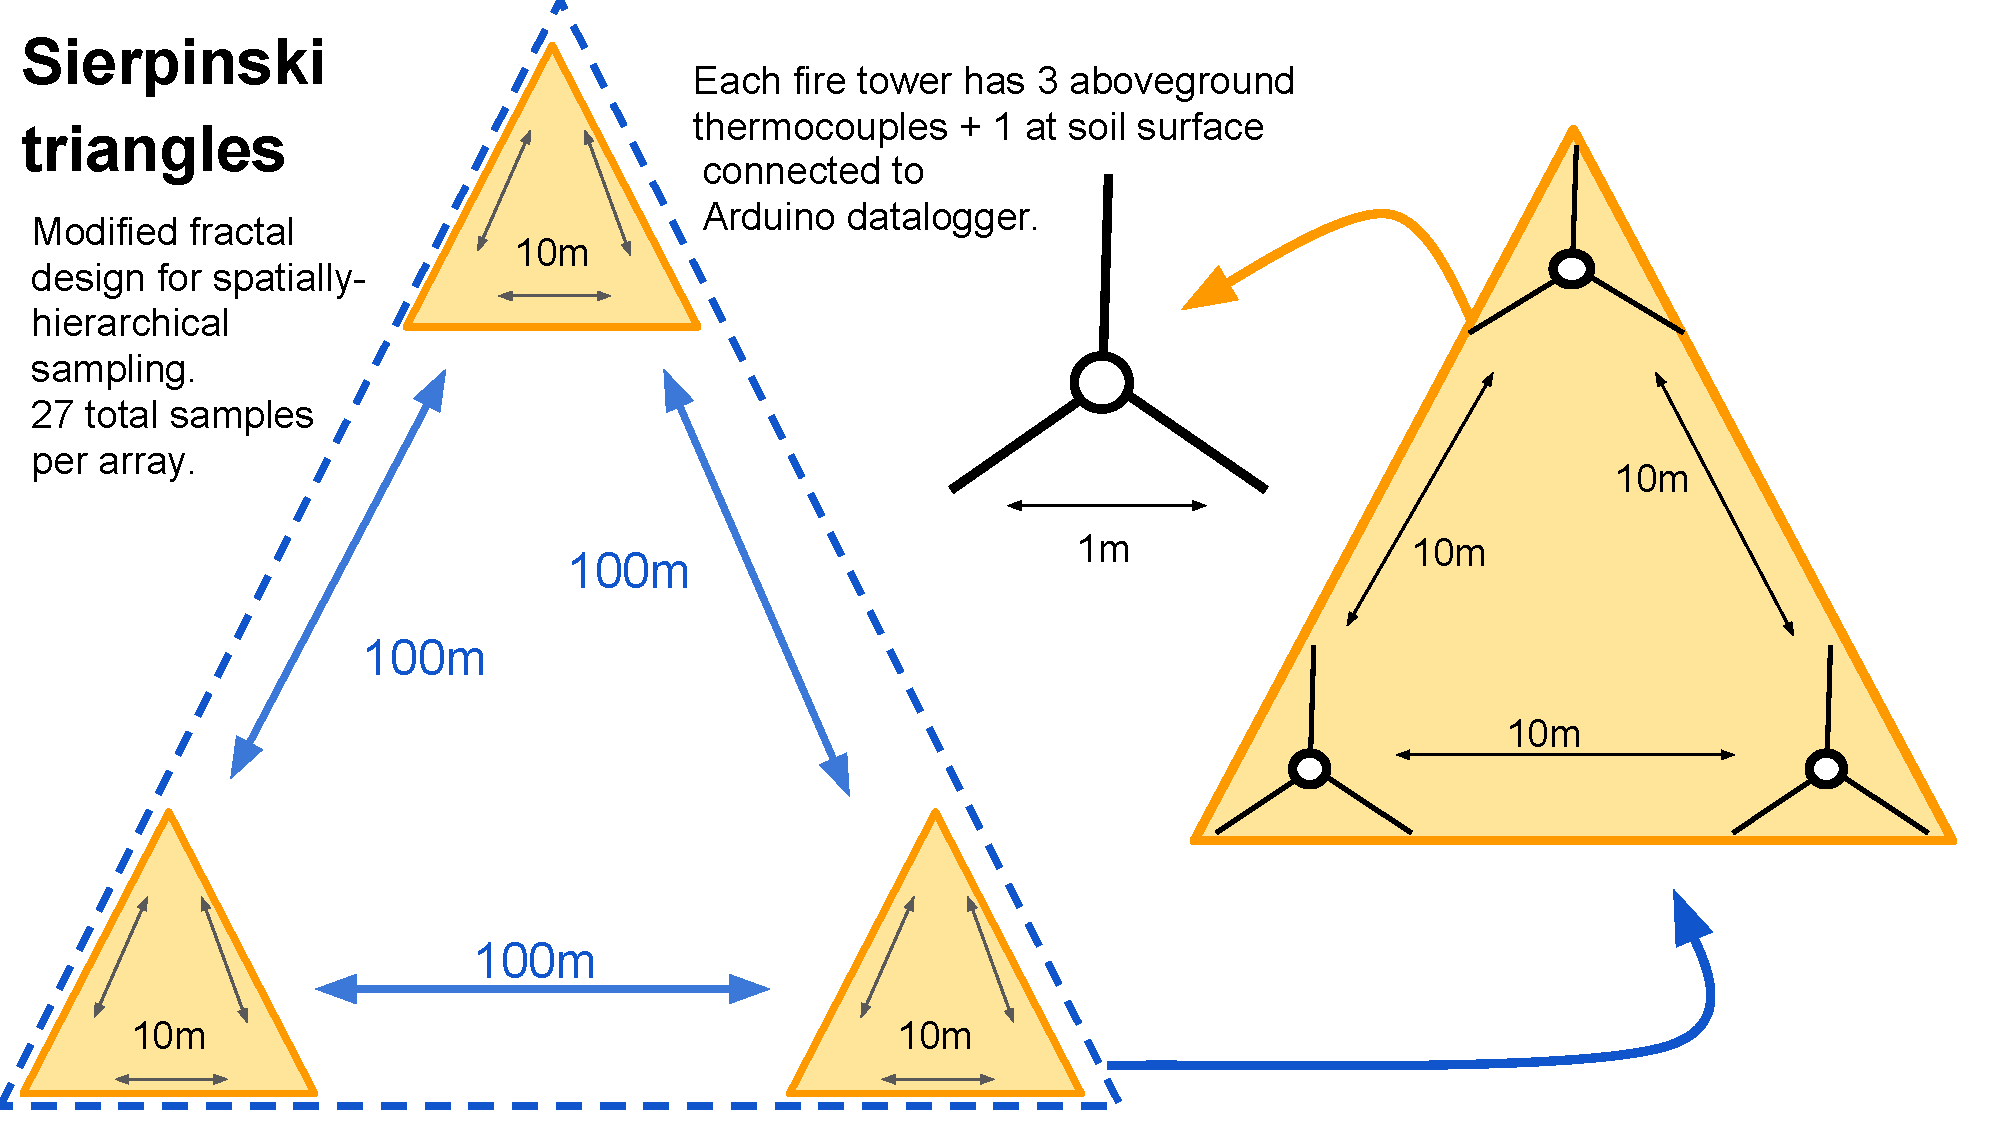
\includegraphics[width=1\linewidth]{figures/SierpinskiTriangle} 

}

\caption{Schematic representation of the Sierpinski Triangle used to deploy 27 thermocouples across 9, 1 m equilateral triangles. Total plot area = 0.433 ha. \label{fig:triangle}}\label{fig:scheme}
\end{figure}

Simard et al.~(1982) describe how rate of spread \(r\) through an
equilateral triangle with sides of length \(D\) can be determined from
the arrival times of the flame front at each point in the triangle
sequentially\textemdash \(t_1\), \(t_2\), and \(t_3\).

If \(t_1 \neq t_2\),

\begin{equation} \label{eq:simard1}
\theta = tan\textsuperscript{-1} \left( \dfrac{2t_3 - t_2 - t_1}{\sqrt{3}\cdot (t_2 - t_1)}\right) 
\end{equation}

and rate of spread \(r\) is

\begin{equation} \label{eq:simard2}
r = \dfrac{D\cdot cos\theta}{t_2 - t_1}
\end{equation}

otherwise, if \(t_1 = t_2\), \(\theta = 90\) and rate of spread \(r\) is

\begin{equation} \label{eq:simard3}
r = D (\sqrt{3}/2)/({t_3 - t_1})
\end{equation}

\hypertarget{additional-results}{%
\section{Additional results}\label{additional-results}}

\hypertarget{fuel-weather-and-fire-behavior-summaries}{%
\subsection{Fuel, weather, and fire behavior
summaries}\label{fuel-weather-and-fire-behavior-summaries}}

\begin{table}[ht]
\centering
\begin{tabular}{lll}
  \hline
Variable & Central Grasslands & Hettinger \\ 
  \hline
Fuel load (kg m$^{-2}$) & 0.2 ± 0.08 & 0.2 ± 0.07 \\ 
  Total fuel moisture (\%) & 32.9 ± 21.58 & 67.9 ± 19.75 \\ 
  Air temperature ($^\circ$C) & 20.3 ± 5.13 & 13.4 ± 5.96 \\ 
  Dew point ($^\circ$C) & 4.4 ± 3.55 & -3.6 ± 7.6 \\ 
  Relative humidity (\%) & 35.9 ± 7.55 & 32.4 ± 9.57 \\ 
  Vapor pressure deficit & 16.3 ± 6.03 & 11.1 ± 4.85 \\ 
  Wind speed (m s$^{-1}$) & 4.3 ± 1.26 & 3.5 ± 1.23 \\ 
  Flame temp ($^\circ$C) & 230 ± 126.33 & 256.4 ± 94.19 \\ 
  Rate of spread (m min$^{-1}$) & 2.1 ± 2.23 & 3.1 ± 2.52 \\ 
  Soil surface temp ($^\circ$C) & 141.2 ± 141.85 & 116.7 ± 131.88 \\ 
   \hline
\end{tabular}
\caption{Summary of fuel, weather, and fire behavior data collected from 25 fires in two locations in North Dakota. Fires in Hettinger were conducted in autumn, while those at Central Grasslands were conducted in spring.} 
\end{table}

\clearpage

\hypertarget{script}{%
\section{Script}\label{script}}

\begin{Shaded}
\begin{Highlighting}[]
\DocumentationTok{\#\#\# S E T U P }
\DocumentationTok{\#\#}
\CommentTok{\# Additional packages required for analysis}
\NormalTok{  pacman}\SpecialCharTok{::}\FunctionTok{p\_load}\NormalTok{(tidyverse, readr, mice, broom.mixed, vegan, lubridate)}
\CommentTok{\# Additional script available via GitHub}
  \FunctionTok{source}\NormalTok{(}\StringTok{\textquotesingle{}https://raw.githubusercontent.com/cran/mice/master/R/mipo.R\textquotesingle{}}\NormalTok{)}
\CommentTok{\#}
\DocumentationTok{\#\#}
\DocumentationTok{\#\#\# D A T A   P R E P A R A T I O N}
\DocumentationTok{\#\#}
\CommentTok{\# Load raw data directly from GitHub}
\NormalTok{  fp }\OtherTok{=} \StringTok{\textquotesingle{}https://raw.githubusercontent.com/devanmcg/SpatialFireBehavior/main\textquotesingle{}}
\CommentTok{\#}
\CommentTok{\# Data wrangling}
\CommentTok{\#}
\NormalTok{ AllData }\OtherTok{\textless{}{-}}  
    \FunctionTok{read\_csv}\NormalTok{(}\FunctionTok{paste0}\NormalTok{(fp, }\StringTok{"/data/fromMZ/CompiledData2.csv"}\NormalTok{)) }\SpecialCharTok{\%\textgreater{}\%}
    \FunctionTok{filter}\NormalTok{(location }\SpecialCharTok{!=} \StringTok{"OAK"}\NormalTok{) }\SpecialCharTok{\%\textgreater{}\%}
      \FunctionTok{mutate}\NormalTok{(}\AttributeTok{date =} \FunctionTok{as.Date}\NormalTok{(date, }\AttributeTok{format =} \StringTok{"\%m/\%d/\%Y"}\NormalTok{),}
               \AttributeTok{L =} \FunctionTok{str\_remove}\NormalTok{(location, }\StringTok{"REC"}\NormalTok{), }
               \AttributeTok{B =} \FunctionTok{str\_sub}\NormalTok{(block, }\DecValTok{1}\NormalTok{,}\DecValTok{3}\NormalTok{), }
               \AttributeTok{Ps =} \FunctionTok{str\_replace}\NormalTok{(pasture, }\StringTok{"[.]"}\NormalTok{, }\StringTok{""}\NormalTok{), }
               \AttributeTok{Ps =} \FunctionTok{str\_sub}\NormalTok{(Ps, }\DecValTok{1}\NormalTok{,}\DecValTok{2}\NormalTok{), }
               \AttributeTok{patch =} \FunctionTok{str\_replace}\NormalTok{(patch, }\StringTok{"[.]"}\NormalTok{, }\StringTok{""}\NormalTok{),}
               \AttributeTok{y =} \FunctionTok{format}\NormalTok{(date, }\StringTok{"\%y"}\NormalTok{)) }\SpecialCharTok{\%\textgreater{}\%}
        \FunctionTok{unite}\NormalTok{(}\StringTok{"FireCode"}\NormalTok{, }\FunctionTok{c}\NormalTok{(L,B,Ps,patch,y), }\AttributeTok{sep=}\StringTok{"."}\NormalTok{) }\SpecialCharTok{\%\textgreater{}\%}
    \FunctionTok{mutate}\NormalTok{(}\AttributeTok{time =} \FunctionTok{str\_remove}\NormalTok{(MaxTempTime, }\StringTok{"[.]+[0{-}9]"}\NormalTok{))}\SpecialCharTok{\%\textgreater{}\%}
    \FunctionTok{unite}\NormalTok{(timestamp, }\FunctionTok{c}\NormalTok{(date, time), }\AttributeTok{sep =} \StringTok{" "}\NormalTok{) }\SpecialCharTok{\%\textgreater{}\%}
    \FunctionTok{mutate}\NormalTok{(}\AttributeTok{timestamp =} \FunctionTok{as.POSIXct}\NormalTok{(timestamp, }\AttributeTok{format =} \StringTok{"\%Y{-}\%m{-}\%d \%H:\%M:\%S"}\NormalTok{)) }\SpecialCharTok{\%\textgreater{}\%}
        \FunctionTok{select}\NormalTok{(FireCode, timestamp, plot, array, TC, MaxC, }
\NormalTok{               AirTemp, RH, dpC, WindSpeed, }
\NormalTok{               LAI, FMC, KgHa) }
\CommentTok{\# Isolate soil surface temperature (TC 4)}
\NormalTok{  SoilTemp }\OtherTok{\textless{}{-}}
    \FunctionTok{filter}\NormalTok{(AllData, TC }\SpecialCharTok{==} \DecValTok{4}\NormalTok{) }\SpecialCharTok{\%\textgreater{}\%}
      \FunctionTok{select}\NormalTok{(FireCode, plot, array, MaxC) }\SpecialCharTok{\%\textgreater{}\%}
        \FunctionTok{rename}\NormalTok{(}\AttributeTok{SoilC =}\NormalTok{ MaxC)}
\CommentTok{\# Summarize array{-}level data }
\NormalTok{  DataMeans }\OtherTok{\textless{}{-}} 
\NormalTok{    AllData }\SpecialCharTok{\%\textgreater{}\%}
      \FunctionTok{filter}\NormalTok{(TC }\SpecialCharTok{\%in\%} \FunctionTok{c}\NormalTok{(}\StringTok{\textquotesingle{}1\textquotesingle{}}\NormalTok{, }\StringTok{\textquotesingle{}2\textquotesingle{}}\NormalTok{, }\StringTok{\textquotesingle{}3\textquotesingle{}}\NormalTok{)) }\SpecialCharTok{\%\textgreater{}\%} 
      \FunctionTok{select}\NormalTok{(}\SpecialCharTok{{-}}\NormalTok{timestamp) }\SpecialCharTok{\%\textgreater{}\%}
      \FunctionTok{pivot\_longer}\NormalTok{(}\AttributeTok{cols =} \FunctionTok{c}\NormalTok{(MaxC}\SpecialCharTok{:}\NormalTok{KgHa), }
                   \AttributeTok{names\_to =} \StringTok{"var"}\NormalTok{,}
                   \AttributeTok{values\_to =} \StringTok{"value"}\NormalTok{) }\SpecialCharTok{\%\textgreater{}\%}
      \FunctionTok{group\_by}\NormalTok{(FireCode, plot, array, var) }\SpecialCharTok{\%\textgreater{}\%}
        \FunctionTok{summarize}\NormalTok{(}\AttributeTok{Mean =} \FunctionTok{mean}\NormalTok{(value) ) }\SpecialCharTok{\%\textgreater{}\%}
      \FunctionTok{ungroup}\NormalTok{() }\SpecialCharTok{\%\textgreater{}\%}
      \FunctionTok{pivot\_wider}\NormalTok{(}\AttributeTok{names\_from =}\NormalTok{ var, }
                  \AttributeTok{values\_from =}\NormalTok{ Mean) }
\CommentTok{\# Calculate Vapor Pressure Deficit}
\NormalTok{  DataMeans }\OtherTok{\textless{}{-}} 
\NormalTok{    DataMeans }\SpecialCharTok{\%\textgreater{}\%}
      \FunctionTok{mutate}\NormalTok{(}\AttributeTok{e  =} \FloatTok{6.11}\SpecialCharTok{*}\NormalTok{(}\DecValTok{10}\SpecialCharTok{\^{}}\NormalTok{((}\FloatTok{7.5}\SpecialCharTok{*}\NormalTok{dpC)}\SpecialCharTok{/}\NormalTok{(}\FloatTok{237.3}\SpecialCharTok{+}\NormalTok{dpC))), }
             \AttributeTok{es =} \FloatTok{6.11}\SpecialCharTok{*}\NormalTok{(}\DecValTok{10}\SpecialCharTok{\^{}}\NormalTok{((}\FloatTok{7.5}\SpecialCharTok{*}\NormalTok{AirTemp)}\SpecialCharTok{/}\NormalTok{(}\FloatTok{237.3}\SpecialCharTok{+}\NormalTok{AirTemp))), }
             \AttributeTok{VPD =}\NormalTok{ es }\SpecialCharTok{{-}}\NormalTok{ e) }\SpecialCharTok{\%\textgreater{}\%}
      \FunctionTok{select}\NormalTok{(}\SpecialCharTok{{-}}\NormalTok{e, }\SpecialCharTok{{-}}\NormalTok{es)}
\CommentTok{\# Calculate rate of spread by arrival time of flame front at sensors }
\NormalTok{  D }\OtherTok{=} \DecValTok{1}   \CommentTok{\# Distance between thermocouples (m)}
\NormalTok{  ROS }\OtherTok{\textless{}{-}} 
\NormalTok{    AllData }\SpecialCharTok{\%\textgreater{}\%}
      \FunctionTok{filter}\NormalTok{(TC }\SpecialCharTok{\%in\%} \FunctionTok{c}\NormalTok{(}\StringTok{\textquotesingle{}1\textquotesingle{}}\NormalTok{, }\StringTok{\textquotesingle{}2\textquotesingle{}}\NormalTok{, }\StringTok{\textquotesingle{}3\textquotesingle{}}\NormalTok{)) }\SpecialCharTok{\%\textgreater{}\%}
      \FunctionTok{mutate}\NormalTok{(}\AttributeTok{timestamp =} \FunctionTok{format}\NormalTok{(timestamp, }\StringTok{"\%H:\%M:\%S"}\NormalTok{), }
             \AttributeTok{ArrivalTime =} \FunctionTok{seconds}\NormalTok{(}\FunctionTok{hms}\NormalTok{(timestamp)) ) }\SpecialCharTok{\%\textgreater{}\%}
    \FunctionTok{select}\NormalTok{(FireCode, plot, array, ArrivalTime) }\SpecialCharTok{\%\textgreater{}\%}
    \FunctionTok{group\_by}\NormalTok{(FireCode, plot, array) }\SpecialCharTok{\%\textgreater{}\%}
    \FunctionTok{arrange}\NormalTok{(ArrivalTime, }\AttributeTok{.by\_group =} \ConstantTok{TRUE}\NormalTok{) }\SpecialCharTok{\%\textgreater{}\%} 
    \FunctionTok{mutate}\NormalTok{(}\AttributeTok{position =} \FunctionTok{order}\NormalTok{(}\FunctionTok{order}\NormalTok{(ArrivalTime, }\AttributeTok{decreasing=}\ConstantTok{FALSE}\NormalTok{)), }
           \AttributeTok{position =} \FunctionTok{recode}\NormalTok{(position, }\StringTok{"1"}\OtherTok{=}\StringTok{"a"}\NormalTok{, }\StringTok{"2"}\OtherTok{=}\StringTok{"b"}\NormalTok{, }\StringTok{"3"}\OtherTok{=}\StringTok{"c"}\NormalTok{), }
           \AttributeTok{ArrivalTime =} \FunctionTok{as.numeric}\NormalTok{(ArrivalTime) }\SpecialCharTok{/}\DecValTok{60}\NormalTok{ ) }\SpecialCharTok{\%\textgreater{}\%} \CommentTok{\# converts to m/min!}
    \FunctionTok{spread}\NormalTok{(position, ArrivalTime)  }\SpecialCharTok{\%\textgreater{}\%}
\NormalTok{    ungroup }\SpecialCharTok{\%\textgreater{}\%} 
    \CommentTok{\# Apply equations from Simard et al. (1984)}
    \FunctionTok{mutate}\NormalTok{( }\AttributeTok{theta\_rad =} \FunctionTok{atan}\NormalTok{((}\DecValTok{2}\SpecialCharTok{*}\NormalTok{c }\SpecialCharTok{{-}}\NormalTok{ b }\SpecialCharTok{{-}}\NormalTok{ a) }\SpecialCharTok{/}\NormalTok{ (}\FunctionTok{sqrt}\NormalTok{(}\DecValTok{3}\NormalTok{)}\SpecialCharTok{*}\NormalTok{(b }\SpecialCharTok{{-}}\NormalTok{ a))), }
            \AttributeTok{ros =} \FunctionTok{case\_when}\NormalTok{(}
\NormalTok{              a }\SpecialCharTok{==}\NormalTok{ b }\SpecialCharTok{\textasciitilde{}}\NormalTok{ (}\FunctionTok{sqrt}\NormalTok{(}\DecValTok{3}\NormalTok{) }\SpecialCharTok{/} \DecValTok{2}\NormalTok{) }\SpecialCharTok{/}\NormalTok{ (c }\SpecialCharTok{{-}}\NormalTok{ a) , }
\NormalTok{              a }\SpecialCharTok{!=}\NormalTok{ b }\SpecialCharTok{\textasciitilde{}}\NormalTok{  (D}\SpecialCharTok{*}\FunctionTok{cos}\NormalTok{(theta\_rad) }\SpecialCharTok{/}\NormalTok{ (b }\SpecialCharTok{{-}}\NormalTok{ a) ) }
\NormalTok{            )) }\SpecialCharTok{\%\textgreater{}\%}
    \FunctionTok{select}\NormalTok{(}\SpecialCharTok{{-}}\NormalTok{a, }\SpecialCharTok{{-}}\NormalTok{b, }\SpecialCharTok{{-}}\NormalTok{c, }\SpecialCharTok{{-}}\NormalTok{theta\_rad)}
\CommentTok{\#}
\CommentTok{\# Create final tibble for analysis }
\CommentTok{\#}
\NormalTok{  AnalysisData  }\OtherTok{\textless{}{-}} 
    \FunctionTok{full\_join}\NormalTok{(DataMeans, ROS) }\SpecialCharTok{\%\textgreater{}\%}
              \FunctionTok{left\_join}\NormalTok{(SoilTemp) }\SpecialCharTok{\%\textgreater{}\%}
      \FunctionTok{filter}\NormalTok{( ros }\SpecialCharTok{\textless{}=} \DecValTok{40}\NormalTok{,       }\CommentTok{\# remove outliers}
\NormalTok{              MaxC }\SpecialCharTok{\textgreater{}=} \DecValTok{40}\NormalTok{) }\SpecialCharTok{\%\textgreater{}\%}  \CommentTok{\# ditto}
      \FunctionTok{rename}\NormalTok{(}\AttributeTok{FuelMoisture =}\NormalTok{ FMC, }
             \AttributeTok{SoilMaxC =}\NormalTok{ SoilC) }\SpecialCharTok{\%\textgreater{}\%}
        \FunctionTok{mutate}\NormalTok{(}\AttributeTok{FuelMoisture =} \FunctionTok{ifelse}\NormalTok{(FuelMoisture }\SpecialCharTok{\textgreater{}=} \DecValTok{0}\NormalTok{, }
\NormalTok{                                      FuelMoisture, }\ConstantTok{NA}\NormalTok{), }
               \AttributeTok{FuelMoisture =}\NormalTok{ FuelMoisture }\SpecialCharTok{*} \DecValTok{100}\NormalTok{) }\SpecialCharTok{\%\textgreater{}\%}
      \FunctionTok{separate}\NormalTok{(FireCode, }\AttributeTok{into =} \FunctionTok{c}\NormalTok{(}\StringTok{"location"}\NormalTok{, }\StringTok{"block"}\NormalTok{, }\StringTok{"pasture"}\NormalTok{, }
                           \StringTok{"patch"}\NormalTok{, }\StringTok{"year"}\NormalTok{), }
               \AttributeTok{remove =}\NormalTok{ F)}
\CommentTok{\#}
\CommentTok{\# Imputing missing values with mice package}
\CommentTok{\#}
  \CommentTok{\# Calculate imputed datasets on scaled data}
\NormalTok{    imp\_sc }\OtherTok{\textless{}{-}}\NormalTok{ AnalysisData }\SpecialCharTok{\%\textgreater{}\%} 
            \FunctionTok{select}\NormalTok{(}\SpecialCharTok{{-}}\NormalTok{LAI, }\SpecialCharTok{{-}}\NormalTok{JD) }\SpecialCharTok{\%\textgreater{}\%}
            \FunctionTok{mutate}\NormalTok{(}\AttributeTok{ros =} \FunctionTok{ifelse}\NormalTok{(ros }\SpecialCharTok{\textgreater{}=} \DecValTok{12}\NormalTok{, }\ConstantTok{NA}\NormalTok{, ros),    }\CommentTok{\# remove outliers}
                   \AttributeTok{tHa =} \FunctionTok{ifelse}\NormalTok{(tHa }\SpecialCharTok{\textgreater{}=} \DecValTok{4}\NormalTok{, }\ConstantTok{NA}\NormalTok{, tHa)) }\SpecialCharTok{\%\textgreater{}\%} \CommentTok{\# ditto}
            \FunctionTok{mutate\_at}\NormalTok{(}\FunctionTok{vars}\NormalTok{(AirTemp}\SpecialCharTok{:}\NormalTok{tHa), }\SpecialCharTok{\textasciitilde{}}\FunctionTok{as.numeric}\NormalTok{(}\FunctionTok{scale}\NormalTok{(., }\AttributeTok{center=}\NormalTok{F))) }\SpecialCharTok{\%\textgreater{}\%}
                      \FunctionTok{mutate}\NormalTok{(}\FunctionTok{across}\NormalTok{(location}\SpecialCharTok{:}\NormalTok{array, as.factor)) }\SpecialCharTok{\%\textgreater{}\%}
                       \FunctionTok{mice}\NormalTok{(}\AttributeTok{m=}\DecValTok{50}\NormalTok{, }\AttributeTok{seed =} \DecValTok{23109}\NormalTok{, }\AttributeTok{print=}\NormalTok{F)}
\CommentTok{\#}
\DocumentationTok{\#\#}
\DocumentationTok{\#\#\#  S T A T I S T I C A L   M O D E L S}
\DocumentationTok{\#\#}
\CommentTok{\#}
\CommentTok{\# Mixed{-}effect regression models on imputed datasets}
\CommentTok{\#}
\CommentTok{\# Rate of spread}
\CommentTok{\#   }
  \CommentTok{\# Fit model }
\NormalTok{    ros\_RH }\OtherTok{\textless{}{-}} 
      \FunctionTok{with}\NormalTok{(imp\_sc, }\FunctionTok{suppressMessages}\NormalTok{(}
\NormalTok{            lme4}\SpecialCharTok{::}\FunctionTok{glmer}\NormalTok{(ros }\SpecialCharTok{\textasciitilde{}}\NormalTok{ RH }\SpecialCharTok{+}\NormalTok{ tHa }\SpecialCharTok{+}
\NormalTok{                              FuelMoisture }\SpecialCharTok{+}\NormalTok{ WindSpeed }\SpecialCharTok{+}
\NormalTok{                              (}\DecValTok{1}\SpecialCharTok{|}\NormalTok{location}\SpecialCharTok{/}\NormalTok{block}\SpecialCharTok{/}\NormalTok{year}\SpecialCharTok{/}\NormalTok{plot), }
                        \AttributeTok{family=}\FunctionTok{Gamma}\NormalTok{(}\AttributeTok{link =} \StringTok{"log"}\NormalTok{), }
                        \AttributeTok{control=}\NormalTok{lme4}\SpecialCharTok{::}\FunctionTok{glmerControl}\NormalTok{(}\AttributeTok{optimizer=}\StringTok{"bobyqa"}\NormalTok{, }
                                      \AttributeTok{optCtrl=}\FunctionTok{list}\NormalTok{(}\AttributeTok{maxfun=}\DecValTok{100000}\NormalTok{)) )) )}
  \CommentTok{\# Get terms}
\NormalTok{    ros\_terms }\OtherTok{\textless{}{-}} 
      \FunctionTok{full\_join}\NormalTok{(}
      \FunctionTok{summary}\NormalTok{(}\FunctionTok{pool}\NormalTok{(ros\_RH)) }\SpecialCharTok{\%\textgreater{}\%} 
        \FunctionTok{as\_tibble}\NormalTok{() }\SpecialCharTok{\%\textgreater{}\%}
        \FunctionTok{rownames\_to\_column}\NormalTok{(}\StringTok{"row"}\NormalTok{), }
      \FunctionTok{confint.mipo}\NormalTok{(}\FunctionTok{pool}\NormalTok{(ros\_RH)) }\SpecialCharTok{\%\textgreater{}\%}
        \FunctionTok{as\_tibble}\NormalTok{() }\SpecialCharTok{\%\textgreater{}\%}
        \FunctionTok{rownames\_to\_column}\NormalTok{(}\StringTok{"row"}\NormalTok{) ) }
\CommentTok{\#    }
\CommentTok{\# Maximum canopy temperature  }
\CommentTok{\#}
  \CommentTok{\# Fit model}
\NormalTok{    canopy\_RH }\OtherTok{\textless{}{-}} 
      \FunctionTok{with}\NormalTok{(imp\_sc, }\FunctionTok{suppressMessages}\NormalTok{(}
\NormalTok{            lme4}\SpecialCharTok{::}\FunctionTok{glmer}\NormalTok{(MaxC }\SpecialCharTok{\textasciitilde{}}\NormalTok{ RH }\SpecialCharTok{+}\NormalTok{ tHa }\SpecialCharTok{+}
\NormalTok{                            FuelMoisture }\SpecialCharTok{+}\NormalTok{ WindSpeed }\SpecialCharTok{+}
\NormalTok{                          (}\DecValTok{1}\SpecialCharTok{|}\NormalTok{location}\SpecialCharTok{/}\NormalTok{block}\SpecialCharTok{/}\NormalTok{year}\SpecialCharTok{/}\NormalTok{plot), }
                        \AttributeTok{family=}\FunctionTok{Gamma}\NormalTok{(}\AttributeTok{link =} \StringTok{"log"}\NormalTok{), }
                        \AttributeTok{control=}\NormalTok{lme4}\SpecialCharTok{::}\FunctionTok{glmerControl}\NormalTok{(}\AttributeTok{optimizer=}\StringTok{"bobyqa"}\NormalTok{, }
                                      \AttributeTok{optCtrl=}\FunctionTok{list}\NormalTok{(}\AttributeTok{maxfun=}\DecValTok{100000}\NormalTok{)) )) )}
  \CommentTok{\# Get terms}
\NormalTok{    canopy\_terms }\OtherTok{\textless{}{-}} 
      \FunctionTok{full\_join}\NormalTok{(}
        \FunctionTok{summary}\NormalTok{(}\FunctionTok{pool}\NormalTok{(canopy\_RH)) }\SpecialCharTok{\%\textgreater{}\%} 
          \FunctionTok{as\_tibble}\NormalTok{() }\SpecialCharTok{\%\textgreater{}\%}
          \FunctionTok{rownames\_to\_column}\NormalTok{(}\StringTok{"row"}\NormalTok{), }
        \FunctionTok{confint.mipo}\NormalTok{(}\FunctionTok{pool}\NormalTok{(canopy\_RH)) }\SpecialCharTok{\%\textgreater{}\%}
          \FunctionTok{as\_tibble}\NormalTok{() }\SpecialCharTok{\%\textgreater{}\%}
          \FunctionTok{rownames\_to\_column}\NormalTok{(}\StringTok{"row"}\NormalTok{) ) }
\CommentTok{\#}
\CommentTok{\# Maximum soil surface temperature  }
\CommentTok{\#}
  \CommentTok{\# Fit model }
\NormalTok{    soil\_RH }\OtherTok{\textless{}{-}} 
      \FunctionTok{with}\NormalTok{(imp\_sc, }\FunctionTok{suppressMessages}\NormalTok{(}
\NormalTok{            lme4}\SpecialCharTok{::}\FunctionTok{glmer}\NormalTok{(}\FunctionTok{log}\NormalTok{(SoilMaxC}\SpecialCharTok{+}\DecValTok{1}\NormalTok{) }\SpecialCharTok{\textasciitilde{}}\NormalTok{ RH }\SpecialCharTok{+}\NormalTok{ tHa }\SpecialCharTok{+}
\NormalTok{                        FuelMoisture }\SpecialCharTok{+}\NormalTok{ WindSpeed }\SpecialCharTok{+}
\NormalTok{                        (}\DecValTok{1}\SpecialCharTok{|}\NormalTok{location}\SpecialCharTok{/}\NormalTok{block}\SpecialCharTok{/}\NormalTok{year}\SpecialCharTok{/}\NormalTok{plot), }
              \AttributeTok{family=}\FunctionTok{Gamma}\NormalTok{(}\AttributeTok{link =} \StringTok{"log"}\NormalTok{), }
              \AttributeTok{control=}\NormalTok{lme4}\SpecialCharTok{::}\FunctionTok{glmerControl}\NormalTok{(}\AttributeTok{optimizer=}\StringTok{"bobyqa"}\NormalTok{, }
                            \AttributeTok{optCtrl=}\FunctionTok{list}\NormalTok{(}\AttributeTok{maxfun=}\DecValTok{100000}\NormalTok{)) )) )}
  \CommentTok{\# Get terms}
\NormalTok{    soil\_terms }\OtherTok{\textless{}{-}} 
      \FunctionTok{full\_join}\NormalTok{(}
        \FunctionTok{summary}\NormalTok{(}\FunctionTok{pool}\NormalTok{(soil\_RH)) }\SpecialCharTok{\%\textgreater{}\%} 
          \FunctionTok{as\_tibble}\NormalTok{() }\SpecialCharTok{\%\textgreater{}\%}
          \FunctionTok{rownames\_to\_column}\NormalTok{(}\StringTok{"row"}\NormalTok{), }
        \FunctionTok{confint.mipo}\NormalTok{(}\FunctionTok{pool}\NormalTok{(soil\_RH)) }\SpecialCharTok{\%\textgreater{}\%}
          \FunctionTok{as\_tibble}\NormalTok{() }\SpecialCharTok{\%\textgreater{}\%}
          \FunctionTok{rownames\_to\_column}\NormalTok{(}\StringTok{"row"}\NormalTok{) ) }
\CommentTok{\#}
\CommentTok{\# Multivariate analysis}
\CommentTok{\#}
  \CommentTok{\# Reduce mids object to tibble   }
\NormalTok{    imp\_raw }\OtherTok{\textless{}{-}} 
      \FunctionTok{complete}\NormalTok{(imp\_sc, }\StringTok{\textquotesingle{}long\textquotesingle{}}\NormalTok{) }\SpecialCharTok{\%\textgreater{}\%}
      \FunctionTok{as\_tibble}\NormalTok{() }\SpecialCharTok{\%\textgreater{}\%}
      \FunctionTok{unite}\NormalTok{(}\StringTok{"TreeID"}\NormalTok{, }\FunctionTok{c}\NormalTok{(location, block, pasture,}
\NormalTok{                        year, plot, array), }\AttributeTok{sep =} \StringTok{"."}\NormalTok{) }\SpecialCharTok{\%\textgreater{}\%}
      \FunctionTok{select}\NormalTok{(}\SpecialCharTok{{-}}\NormalTok{patch, }\SpecialCharTok{{-}}\NormalTok{.id, }\SpecialCharTok{{-}}\NormalTok{.imp, }\SpecialCharTok{{-}}\NormalTok{FireCode) }\SpecialCharTok{\%\textgreater{}\%}
      \FunctionTok{pivot\_longer}\NormalTok{(}\AttributeTok{names\_to =} \StringTok{"response"}\NormalTok{, }
                   \AttributeTok{values\_to =} \StringTok{"values"}\NormalTok{, }
                   \SpecialCharTok{{-}}\NormalTok{TreeID) }\SpecialCharTok{\%\textgreater{}\%}
      \FunctionTok{group\_by}\NormalTok{(TreeID, response) }\SpecialCharTok{\%\textgreater{}\%}
      \FunctionTok{summarize}\NormalTok{(}\AttributeTok{value =} \FunctionTok{median}\NormalTok{(values)) }\SpecialCharTok{\%\textgreater{}\%}
      \FunctionTok{ungroup}\NormalTok{() }\SpecialCharTok{\%\textgreater{}\%}
      \FunctionTok{pivot\_wider}\NormalTok{(}\AttributeTok{names\_from =}\NormalTok{ response, }
                  \AttributeTok{values\_from =}\NormalTok{ value) }\SpecialCharTok{\%\textgreater{}\%}
      \FunctionTok{separate}\NormalTok{(TreeID, }\FunctionTok{c}\NormalTok{(}\StringTok{"location"}\NormalTok{, }\StringTok{"block"}\NormalTok{, }\StringTok{"pasture"}\NormalTok{,}
                         \StringTok{"year"}\NormalTok{, }\StringTok{"plot"}\NormalTok{, }\StringTok{"array"}\NormalTok{)) }\SpecialCharTok{\%\textgreater{}\%} 
      \FunctionTok{mutate}\NormalTok{(}\FunctionTok{across}\NormalTok{(location}\SpecialCharTok{:}\NormalTok{array, as.factor))}
  \CommentTok{\# Fire behavior PCA }
\NormalTok{    fb\_d }\OtherTok{\textless{}{-}} 
\NormalTok{      imp\_raw }\SpecialCharTok{\%\textgreater{}\%}
      \FunctionTok{select}\NormalTok{(MaxC, ros, SoilMaxC) }
\NormalTok{    fb\_pca }\OtherTok{\textless{}{-}} \FunctionTok{rda}\NormalTok{(fb\_d }\SpecialCharTok{\textasciitilde{}} \DecValTok{1}\NormalTok{, }\StringTok{\textquotesingle{}euc\textquotesingle{}}\NormalTok{, }\AttributeTok{scale =}\NormalTok{ T)}
  \CommentTok{\# Test differences between locations }
    \FunctionTok{envfit}\NormalTok{(fb\_pca }\SpecialCharTok{\textasciitilde{}}\NormalTok{ location, imp\_raw, }
           \AttributeTok{choices =} \FunctionTok{c}\NormalTok{(}\DecValTok{1}\SpecialCharTok{:}\DecValTok{2}\NormalTok{), }
           \AttributeTok{strata =}\NormalTok{ imp\_raw}\SpecialCharTok{$}\NormalTok{year, }
           \DecValTok{199}\NormalTok{)}\SpecialCharTok{$}\NormalTok{factors}
\CommentTok{\# Test fire weather against PCA}
   \FunctionTok{envfit}\NormalTok{(fb\_pca }\SpecialCharTok{\textasciitilde{}}\NormalTok{ MaxWindSpeed}\SpecialCharTok{+}\NormalTok{AirTemp}\SpecialCharTok{+}\NormalTok{dpC}\SpecialCharTok{+}\NormalTok{RH}\SpecialCharTok{+}\NormalTok{VPD, }
          \AttributeTok{data =}\NormalTok{ imp\_raw, }
          \AttributeTok{choices =} \FunctionTok{c}\NormalTok{(}\DecValTok{1}\SpecialCharTok{:}\DecValTok{3}\NormalTok{), }
          \AttributeTok{strata =}\NormalTok{ imp\_raw}\SpecialCharTok{$}\NormalTok{location)}
\end{Highlighting}
\end{Shaded}


\end{document}
